\chapter{Desarrollo}

El desarrollo del juego se puede separar en tres grandes bloques diferentes entre s�: Dise�o, arte y programaci�n.


%----- Dise�o --------------------------------------
%---------------------------------------------------
\section{Dise�o}


%----- Arte ----------------------------------------
%---------------------------------------------------
\section{Arte}

%----- Programaci�n --------------------------------
%---------------------------------------------------
\section{Programaci�n}

\subsection{Gr�ficos}

\subsection{C�mara}

\subsection{F�sica}

\subsection{Inteligencia Artificial}

\subsubsection{M�quinas de estados}

\subsubsection{Steering Behaviors}

\subsection{Scripting}

\subsection{Audio}

Para la gesti�n de sonido y m�sica se ha utilizado la librer�a Wwise \cite{wwise} de Audiokinetic. La librer�a es de pago menos para Windows que es gratuita si el producto final es de uso no comercial. Wwise se utiliza en multitud de juegos actuales, entre ellos \emph{Mass Effect 3} \cite{ME3}, \emph{Assassin's Creed II} \cite{AC2}, \emph{inFamous 2} \cite{infamous} y \emph{Batman: Arkham City} \cite{batman}, entre otros.

Wwise funciona mediante eventos y bancos de sonido. En los bancos de sonido es donde residen todas las pistas de audio y los eventos son instrucciones sobre las pistas de audio. La creaci�n de estos dos elementos se hace mediante el editor que lleva la propia librer�a (figura \ref{fig:wwise_editor}).

\begin{figure}
\begin{center}
\includegraphics[scale=0.35]{figures/development/wwise_editor.eps}
\end{center}
\emph{\caption{Editor de Wwise con el proyecto del juego}\label{fig:wwise_editor}}
\end{figure}

Tambi�n se ha hecho uso de los RTPCs (\emph{Real-Time Parameter Controls}). Los RTPCs son curvas asociadas a un audio que, a partir de un par�metro, se puede modificar el sonido en tiempo real. Se han utilizado para poder modificar el volumen del sonido y de la m�sica en cualquier momento. 

\subsection{Tools}

Se han hecho diferentes herramientas para el f�cil y �gil desarrollo de algunas partes del juego. As� pues, se han hecho la herramientas: Particle Editor, GUI Editor y 3ds Max Exporter.

\subsubsection{Particle Editor} \label{sec:particleeditor}
Durante el desarrollo del juego, se ha llevado a cabo un simple editor de part�culas (figura \ref{fig:particle_editor}) para poder generar las part�culas de una forma m�s �gil, r�pida y visual. Est� hecho con MFC (\emph{Microsoft Foundation Class}).

El editor permite modificar todos los par�metros de un sistema de part�culas en tiempo real. Al mismo tiempo, se puede ejecutar el sistema de part�culas creado en diferentes tipos de emisores (tipo punto, caja, esfer, anillo, l�nea).

La herramienta permite generar sistemas de part�culas distintos y guardarlos en un fichero XML preparado para ser le�do directamente por el motor del juego.

\begin{figure}
\begin{center}
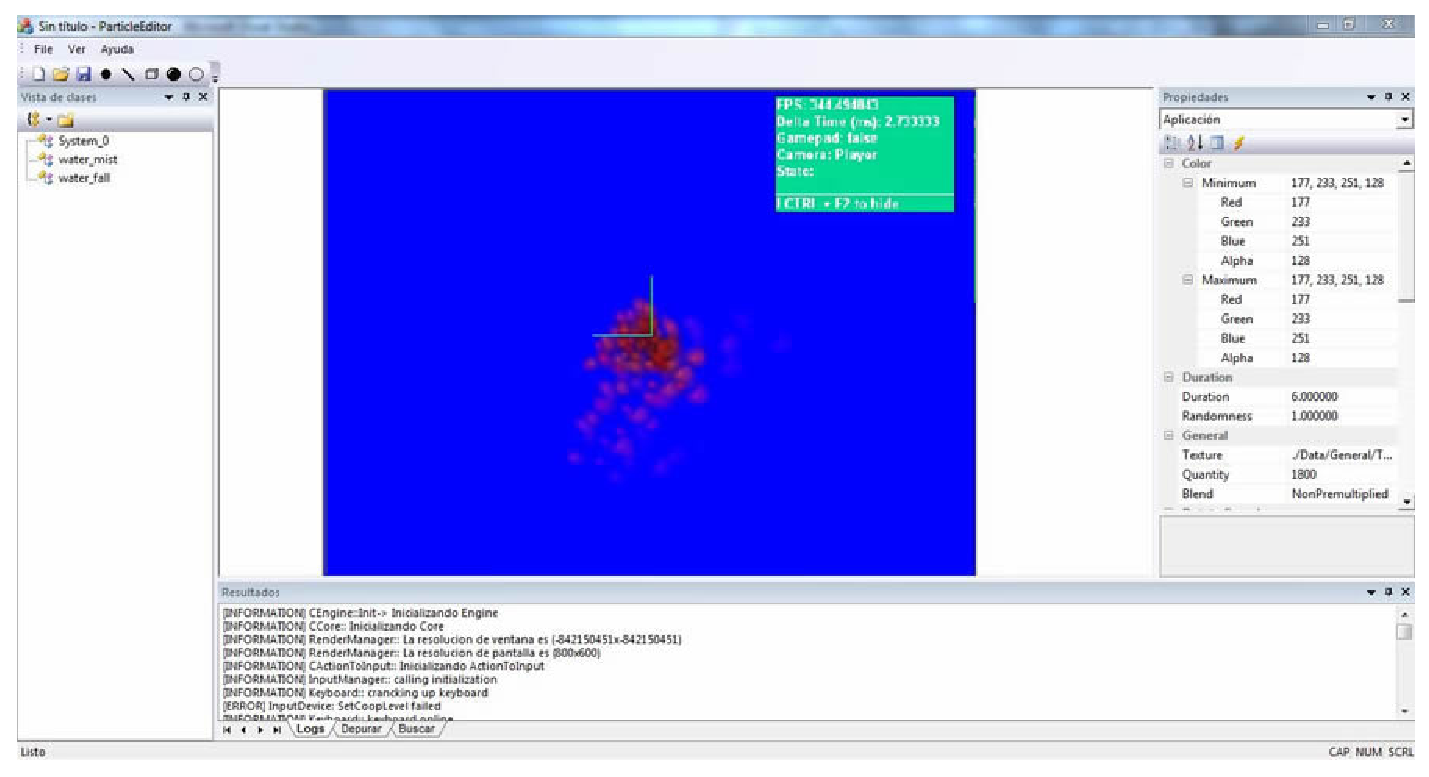
\includegraphics[scale=0.5]{figures/development/particle_editor.eps}
\end{center}
\emph{\caption{Particle Editor}\label{fig:particle_editor}}
\end{figure}

\subsubsection{GUI Editor}

Se ha desarrollado un editor (figura \ref{fig:gui_editor}) para poder hacer los men�s del juego de una forma senzilla y r�pida. Como el \emph{Particle Editor} (secci�n \ref{sec:particleeditor}), est� hecho con MFC.

El editor permite poner todos los controles de los que dispone (botones, im�genes,...) mediante \emph{drag and drop}. Adem�s, se puede modificar las propiedades de todos los controles que conforman la ventana, pudiendo personalizar totalmente la ventana de una forma visual.

La herramienta permite generar ventanas para trabajar con toda la GUI del juego a la vez y, tambi�n, guardar toda la informaci�n en ficheros XML que son le�dos por el motor.

\begin{figure}
\begin{center}
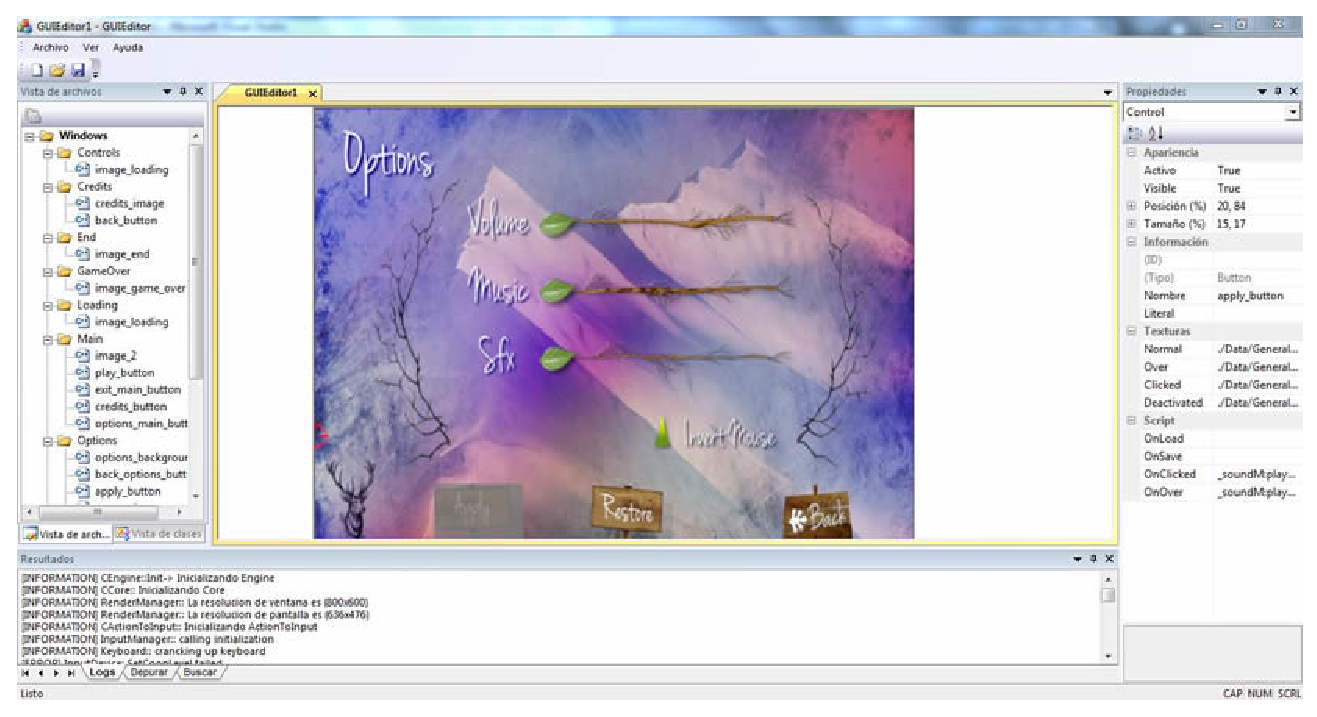
\includegraphics[scale=0.5]{figures/development/gui_editor.eps}
\end{center}
\emph{\caption{GUI Editor}\label{fig:gui_editor}}
\end{figure}

\subsubsection{3ds Max Exporter}


